%%%%%%%%%%%%%%%%%%%%%%%%%%%%%%%%%
%Preamble
%%%%%%%%%%%%%%%%%%%%%%%%%%%%%%%%%

\documentclass[a4paper]{article}
\usepackage[english]{babel}
\usepackage[margin=1in]{geometry}
\usepackage[ruled, vlined]{algorithm2e}

\usepackage{amsfonts}
\usepackage{setspace,graphicx,epstopdf,amsmath}
\usepackage{marginnote, datetime, url, enumitem, subfigure}

%Journal Style
%JFE looks nice, JF looks awful
\usepackage{amsthm}
\usepackage{jfe}

%Bibliography Stuff
%Use natbib even though it's old because it's compliant with journal styles
%Actual bibliography style etc are specified where you actually want it
\usepackage{natbib}

%Fluff
\linespread{1.3}

%Neural Network Packages
\usepackage{neuralnetwork}
\usepackage{xpatch}
\makeatletter
% \linklayers have \nn@lastnode instead of \lastnode,
% patch it to replace the former with the latter, and similar for thisnode
\xpatchcmd{\linklayers}{\nn@lastnode}{\lastnode}{}{}
\xpatchcmd{\linklayers}{\nn@thisnode}{\thisnode}{}{}
\makeatother

%Regression Tree
\usepackage{tikz,forest}
\usetikzlibrary{arrows.meta}

\forestset{
	.style={
		for tree={
			base=bottom,
			child anchor=north,
			align=center,
			s sep+=1cm,
			straight edge/.style={
				edge path={\noexpand\path[\forestoption{edge},thick,-{Latex}] 
					(!u.parent anchor) -- (.child anchor);}
			},
			if n children={0}
			{tier=word, draw, thick, rectangle}
			{draw, diamond, thick, aspect=2},
			if n=1{%
				edge path={\noexpand\path[\forestoption{edge},thick,-{Latex}] 
					(!u.parent anchor) -| (.child anchor) node[pos=.2, above] {Y};}
			}{
				edge path={\noexpand\path[\forestoption{edge},thick,-{Latex}] 
					(!u.parent anchor) -| (.child anchor) node[pos=.2, above] {N};}
			}
		}
	}
}

%%TODONOTE commands
\usepackage[colorinlistoftodos]{todonotes}
\newcommand{\smalltodo}[2][] {\todo[caption={#2}, size=\scriptsize,%
	fancyline,#1]{\begin{spacing}{.5}#2\end{spacing}}}
\newcommand{\rhs}[2][]{\smalltodo[color=green!30,#1]{{\bf RS:} #2}}
%%

%Graphs
\usepackage{tikz}
\usepackage{pgfplots}

%Coloured Tables


%%%%%%%%%%%%%%%%%%%%%%%%%%%%%%
%%Title and other fluff, just before document start
%%%%%%%%%%%%%%%%%%%%%%%%%%%%%%

%Hyperref apparently is a big package and causes a lot of issues, so it's recommended to load this last

\usepackage{hyperref}

%Gets rid of the neon green boxes around boxes

\usepackage{xcolor}
\hypersetup{
	colorlinks,
	linkcolor = {red!50!black},
	citecolor = {blue!50!black},
	urlcolor = {blue!80!black}
}

\title{Evaluation of Machine Learning in Empirical Asset Pricing}
\author{Ze Yu Zhong}

%%%%%%%%%%%%%%%%%%%%%%%%%%%%%%%
%%BEGIN DOCUMENT
%%%%%%%%%%%%%%%%%%%%%%%%%%%%%%%

\begin{document}
	
	\maketitle
	
	%\listoftodos
	
	%\tableofcontents
	
	\section{Introduction}
	
	\subsection{Topic}
	
	This thesis aims to evaluate the application of machine learning algorithms in empirical asset pricing. While there has been a significant recent interest in applying machine learning to the problem of predicting asset returns, there is little literature that focuses on how well these algorithms are at capturing true underlying mechanisms of stock returns. 12 different simulated datasets ranging from linear to highly non-linear data generating processes incorporating observed phenomena of cross sectional correlation, persistence, endogeneity, stochastic volatility, and real world data will be used to assess the performance of linear models, elastic net models, random forests and neural networks.
	
	\subsection{Background Literature and Motivations}
	
	This paper is motivated by evaluating the performance of machine learning algorithms in empirical asset pricing, focusing on how well they deal with the many unique problems in financial returns data.
	
	Financial returns data exhibits many problems for statistical analysis: regressors are numerous and display persistence, non-stationarity, cross sectional correlation and endogeneity, in addition to the overall high noise (randomness) in financial returns data. Furthermore, the characteristics of financial data has not remained similar over time, presenting an additional non-robustness problem. Numerous examples of these  controversies surrounding factors have plagued the literature. For example, company valuation ratios such as dividend yield were introduced despite their validity being contingent on being a stationary time series, for which there was mixed evidence even when introduced, \citep{vuolteenaho_understanding_1999}. Though models incorporating dividend yield initially performed well, they were later shown to seemingly break down in a changing economic environment, (\cite{lettau_consumption_2001}, \cite{schwert_anomalies_2003} and others).
	
	This has not stopped the literature searching for more factors: quantitative trading firms were using 81 factor models as the norm \citep{hsu_finding_2014} by 2014, and literature has emerged in trying to evaluate the "factor zoo" consisting of well over 600 factors, (\cite{harvey__2016}, \cite{harvey_census_2019}, among others).
	
	Much of the literature developing models to try to deal with problematic regressors. To this end, machine learning algorithms have emerged and been recognised as well suited: algorithms such as shrinkage and selection methods have been utilised in factor selection (\cite{kozak_shrinking_2017}, \cite{rapach_forecasting_2013}, \cite{freyberger_dissecting_2017}), and most importantly, portfolios constructed using machine learning have been demonstrated to outperform traditional models in predicting stock returns (\cite{gu_empirical_2018}, \cite{hsu_finding_2014}, \cite{feng_deep_2018}). This has been attributed to machine learning's ability to evaluate and consider non-linear complexities among factors that cannot be feasibly achieved using traditional techniques.  
	
	However, though machine learning has shown great promise in these areas, little work done on how machine learning actually recognises and deals with the aforementioned problems in returns data. Prior work been done by \cite{gu_empirical_2018}, however; only basic simulation designs which did not fully explore these problems were used.
	
	This paper will be the first in focusing on how machine learning algorithms perform in environments with problems exhibited by financial returns data through extensive simulations. In addition, these algorithms will once again be evaluated on real world data, but with only more recent and representative data included in order to test their short term robustness in predicting stock returns. These two aspects of the study together are able to offer a better glimpse as to how ``black box" machine learning algorithms deal with the challenges present in asset pricing, if at all.
	
	%\subsection{Limitations of Machine Learning}
	
	%Machine learning excels at prediction problems, namely estimating \( E(r_{i, t+1}|\mathcal{F}_t) \), where \( r_{i, t+1} \) is an asset's excess return over the risk free rate, and \( \mathcal{F}_t \) is the set of all information (including unobservable) available to market participants in this context.
	
	%This means that machine learning algorithms do not, nor do they aim to, explain how the market works in terms of underlying dynamics and equilibria. Though a machine learning algorithm may be able to identify patterns that otherwise cannot be easily found, an economist is still required to analyse these patterns to construct and hypothesize economic theory.
	
	\section{Methodology}
	
	\subsection{Overall Model Design}
	
	Each model will be presented and explained so that a reader without any machine learning background can understand the basic idea behind each model. Details such as the computational and specific algorithm used for each model are included in the Appendix (\ref{Algorithms}). This is because there are many variations of algorithms available, and more importantly, specific understanding of how the algorithm works is not necessary. 
	
	All asset excess returns are modelled as an additive prediction error model:
	
	\begin{equation}
	r_{i, t+1} = E(r_{i, t+1} | \mathcal{F}_t) + \epsilon_{i, t+1}
	\end{equation}
	
	where 
	
	\begin{equation}
	E(r_{i, t+1} | \mathcal{F}_t) = g^*(z_{i,t})
	\end{equation}
	
	with $g^*(z_{i,t})$ representing the model approximation using the predictor set $z_{i,t}$.
	
	\subsection{Sample Splitting}
	
	Imperative to any machine learning technique is the establishment of how the dataset is to be split into training, validation and test sets. The training set is used to initially build the model and provide initial estimates of parameters, whereas the validation set is used to tune model parameters to optimise out of sample performance, thus preventing overfitting. The validation set acts as a simulation of out of sample testing, whereas the test set is used only for evaluation, and is thus truly out of sample.
	
	There are three main approaches to splitting temporal data (such as financial data). 
	
	The first is to decide arbitrarily on a single training, validation and test set. This method is straightforward and the least computationally intensive, but is limited and inflexible in evaluating how models perform when more recent data is provided for training. 
	
	The second method is a "rolling window" method, where a fixed size or "window" for the training and validation set is first chosen. This window then incrementally move forwards in time to include more recent data, with a set of forecasts for the test sets made for all possible windows.
	
	The third is a "recursive" method, which is the same as the rolling window method, but different in that the training set always contains previous data, with only the validation set staying fixed in size and "rolling" forwards. Hence, it is also referred to as a "growing window."
	
	Both the rolling window and recursive schemes are very computationally intensive. Therefore, a hybrid of the rolling and recursive schemes was considered: the training set is increased by one year with each refit, the validation set remains one year in length but moves forward by one year, and forecasts are made using that model for the subsequent year. Cross validation was not done to maintain the temporal ordering of the data.
	
	\subsection{Loss Function}
	
	The choice of the loss function used in models is imperative to machine learning. The loss functions considered are Mean Absolute Error (MAE), Mean Squared Error and Root Mean Squared Error (MSE, and RMSE) and Huber Loss.
	
	\subsubsection{Mean Absolute Error}
	
	The mean absolute error (MAE) is simply the average magnitude of errors. Because of this, it places equal weighting to all magnitudes of errors and is more robust to outliers. Limitations of this metric are its non-differentiability when the error is 0 (see Figure \ref{fig:loss_functions}).
	
	\begin{equation}
	\text{MAE} = \frac{1}{n} \sum_{j = i}^{n} |y_j - \hat{y_j}|
	\end{equation}
	
	\subsubsection{Mean Squared Error and Root Mean Squared Error}
	
	The mean squared error (MSE) and root mean squared error (RMSE) are quadratic scoring methods. This means that they place higher weight on large errors. Models that minimize this metric are therefore more sensitive to outliers. 
	
	\begin{align}
	\text{MSE} &= \frac{1}{n} \sum_{j = i}^{n} \left( y_j - \hat{y_j}\right) ^2 \\
	\text{RMSE} &= \sqrt{ \frac{1}{n} \sum_{j = i}^{n} \left( y_j - \hat{y_j}\right) ^2}
	\end{align}
	
	\subsubsection{Huber Loss}
	
	The Huber Loss metric \citep{huber_robust_1992} offers a combination of mean squared error and mean absolute error, with errors smaller than the threshold $\xi$ being mean squared error and errors larger than the threshold $\xi$ being absolute error. This allows for the model fit to be less sensitive to outliers which are quite common in financial data. 
	
	\begin{align}
	H(\epsilon_j = y_j - \hat{y_j};\xi) = 
	\begin{cases}
	\left( y_j - \hat{y_j}\right) ^2, 
	\quad &\text{if} \quad |y_j - \hat{y_j}| \leq \xi ; \\
	2 \xi  |y_j - \hat{y_j}| - \xi^2, 
	\quad &\text{if} \quad |y_j - \hat{y_j}| > \xi
	\end{cases}
	\end{align}
	
	\begin{figure}
		\begin{center}
			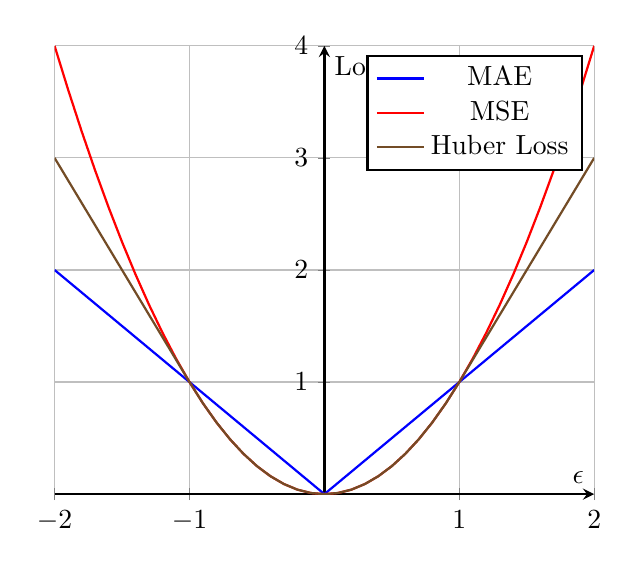
\begin{tikzpicture}
			\begin{axis}[ xlabel={$\epsilon$}, ylabel={Loss}, axis lines=middle, samples=41, grid, thick, domain=-2:2]
			\addplot+[no marks] {abs(x)};
			\addlegendentry{MAE}
			\addplot+[no marks] {x^2};
			\addlegendentry{MSE}
			\addplot+[no marks] {(2 * abs(x) - 1)*(abs(x) > 1) +
				(x^2)*(abs(x) <= 1 )};
			\addlegendentry{Huber Loss}
			\end{axis}
			\end{tikzpicture}
		\end{center}
		\caption{Illustration of MAE, MSE and Huber Loss when $\xi = 1$}
		\label{fig:loss_functions}
	\end{figure}
	
	\subsection{Linear Model}
	
	The least complex model considered is the simple linear regression model, also known that ordinary least squares in the case of the using mean squared error as the loss function. Linear models struggle with high-dimensionality. Nevertheless, despite being expected to perform poorly it was implemented as a ``control."
	
	The simple linear model assumes that the underlying conditional expectation \( g^*(z_{i, t}) \) can be modelled as a linear function of the predictors and the parameter vector \( \theta \):
	
	\begin{equation}
	g(z_{i, t};\theta) = z_{i, t}' \theta
	\end{equation}
	
	This model can capture non-linearities only if the predictor set \(z^*_{i, t}\) contains specified non-linear transformations or interaction terms. 
	
	Computing this model with respect to minimizing the mean squared error yields the pooled ordinary least squares estimator (POLS).
	
	\subsection{Penalized Linear Model}
	
	Penalized linear models have the same underlying statistical model as simple linear models, but differ in their addition of a new penalty term in the loss function:
	
	\begin{equation}
		\mathcal{L(\theta;.)} = 
		\underset{\text{Loss Function}}{\underbrace{\mathcal{L(\theta)}}} + 
		\underset{\text{Penalty Term}}{\underbrace{\phi(\theta;.)}}
	\end{equation}
	
	Several choices exist for the choice of the penalty function \( \phi(\theta;.) \). This focus of this paper is the popular "elastic net" penalty  \citep{zou_regularization_2005}, which takes the form:
	
	\begin{equation}
		\phi(\theta;\lambda,\rho) = 
		\lambda(1-\rho) \sum_{j = 1}^{P}|\theta_j| +
		\frac{1}{2} \lambda \rho \sum_{j = 1}^{P}\theta_j^2
	\end{equation}
	
	The elastic net has two hyperparameters: $\lambda$, which controls the overall magnitude of the loss, and $\rho$, which controls the shape of the penalization. The $\rho = 0$ case corresponds to the popular LASSO and uses absolute ($l_1$) parameter penalization, which geometrically allows the coefficients to be shrunk to 0. This allows it to impose sparsity, and can be thought of as a variable selection tool.
	
	The $\rho = 1$ case corresponds to ridge regression, which uses $l_2$ that shrinks all coefficients closer to 0, but not to 0. Ridge regression is therefore a shrinkage method which prevents coefficients from becoming too large and overpowering. For \(0 < \rho < 1\), the elastic net aims to produce parsimonious models through both shrinkage and selection.
	
	The hyperparameters $\lambda$ and $\rho$ are both tuned using the validation sample (see \ref{Algorithms})
	
	\subsection{Classification and Regression Trees}
	
	Classification and regression trees are fully non-parametric models that can capture complex multi-way interactions. A tree "grows" in a series of iterations. With each iteration, a split ("branch") is made along one predictor such that it is the best split available at that stage with respect to minimizing the loss function. These steps are continued until each observation is its own node, or more commonly until the stopping criterion is met. The eventual model slices the predictor space into rectangular partitions, and predicts the unknown function $g^*(z_{i,t})$ with the average value of the outcome variable in each partition.
	
	The prediction of a tree, $\mathcal{T}$, with \(K\) "leaves" (terminal nodes), and depth $L$ is
	
	\begin{equation}
	g(z_{i,t};\theta,K,L) = \sum_{k=1}^{K}\theta_k\textbf{1}_{z_{i,t}\in C_k(L)}
	\end{equation}
	
	where $C_k(L)$ is one of the $K$ partitions in the model.
	
	For this study, only recursive binary trees (the most common and easy to implement ) are considered. Though trees were originally proposed and fit with respect to minimizing mean squared error, they can be grown with respect to a variety of loss functions, including mean absolute error, mean squared error and Huber Loss:
	
	\begin{equation}
	H(\theta, C) = \frac{1}{|C|} \sum_{z_{i,t} \in C} L(r_{i,t+1} - \theta)
	\end{equation}
	
	where $|C|$ denotes the number of observations in set C (partition). Given $C$, it is clear that the optimal choice for minimising the loss function when it is mean squared error is simply $\theta = \frac{1}{|C|} \sum_{z_{io,t}\in C}^{ }r_{i,t+1}$ i.e. the average of the partition, and the median of the partition when the loss function is mean absolute error.
	
	Trees, grown to a deep enough level, are highly unbiased and flexible. The tradeoff of course, is their high variance and instability. Thus, an ensemble method called "Random Forest" was proposed to regularize trees by combining many different trees into a single prediction.
	
	\subsection{Random Forests}
	Random Forests are an extension of trees that attempt to address some of their problems. A random forest algorithm creates $B$ different bootstrap samples from the training dataset, fits an overfit (and hence low bias) regression tree to each using only a random subset $m$ size from all available predictors (also known as dropout), and then averages their forecasts as the final output. The overfit trees means that the underlying trees has low bias, and the dropout procedure means that they have low correlation. Thus, averaging these low bias, uncorrelated trees results in a low bias, yet stable model. Specific details of the random forest algorithm are detailed in the appendix.
	
	\pagebreak
	
	\subsection{Neural Networks}
	
	\subsubsection{Introduction}
	
	Neural networks are arguably the most complex type of model available, able to capture several non-linear interactions through their many layers, hence its other name ``deep learning." On the flipside, their high flexibility often means that they are among the most parameterized and least interpretable models, earning them the reputation as a black box model.
	
	The scope of this paper is limited to traditional ``feed-forward" networks. The feed forward network consists of an ``input layer" of scaled data inputs, one or more ``hidden layers" which interact and non-linearly transform the inputs, and finally an output layer that aggregates the hidden layers and transform them a final time for the final output. 
	
	Neural networks with up to 5 hidden layers were considered, each named NNX where X represents the number of hidden layers. The number of neurons is each layer was chosen according to the geometric pyramid rule \citep{masters_practical_1993}: NN1 has 32 neurons, NN2 has 32 and 16 neurons in the first and second hidden layers respectively, NN3 has 32, 16, and 8 neurons, NN4 has 32, 16, 8, and 4 neurons, and NN5 has 32, 16, 8, 4, 2 neurons respectively. All units are fully connected; that is, each neurons receives input from all neurons the layer before it (see Figure \ref{Neural_Network}).
	
	\begin{figure}
		\begin{center}
			\begin{neuralnetwork}
				%Options
				[nodespacing=12mm, layerspacing=20mm,
				maintitleheight=2.5em, layertitleheight=2.5em,
				height=8, toprow=false, nodesize=20pt, style={},
				title={}, titlestyle={}]
				\newcommand{\nodetextclear}[2]{}
				%use \ifnum to get different labels, such as x_n on the last neuron
				\newcommand{\nodetextx}[2]{\ifnum #2=8 $x_n^{(0)}$ \else $x_#2^{(0)}$ \fi}
				\newcommand{\nodetexty}[2]{$y_#2$}
				%Hidden layer textcommands
				%32 neurons
				\newcommand{\nodetextxa}[2]{\ifnum #2=7 $x_{32}^{(1)}$ \else $x_#2^{(1)}$ \fi}
				%16 neurons
				\newcommand{\nodetextxb}[2]{\ifnum #2=6 $x_{16}^{(2)}$ \else $x_#2^{(2)}$ \fi}
				%8 neurons
				\newcommand{\nodetextxc}[2]{\ifnum #2=5 $x_{8}^{(3)}$ \else $x_#2^{(3)}$ \fi}
				\newcommand{\nodetextxd}[2]{$x_#2^{(4)}$}
				\newcommand{\nodetextxe}[2]{$x_#2^{(5)}$}
				%Input Layer
				\inputlayer[count=8, bias=false, exclude = {7}, title=Input Layer, text=\nodetextx]
				%Hidden Layer 1
				\hiddenlayer[count=7, bias=false, exclude = {6}, title=Hidden Layer 1, text=\nodetextxa] 
				\linklayers[not from = {7}, not to = {6}]
				%Hidden Layer 2
				\hiddenlayer[count=6, bias=false, exclude = {5}, title=Hidden Layer 2, text=\nodetextxb] 
				\linklayers[not from = {6}, not to = {5}]
				%Hidden Layer 3
				\hiddenlayer[count=5, bias=false, exclude = {4}, title=Hidden Layer 3, text=\nodetextxc] 
				\linklayers[not from = {5}, not to = {4}]
				%Hidden Layer 4
				\hiddenlayer[count=4, bias=false, title=Hidden Layer 4, text=\nodetextxd] 
				\linklayers[not from = {4}]
				%Hidden Layer 5
				\hiddenlayer[count=2, bias=false, title=Hidden Layer 5, text=\nodetextxe] \linklayers
				%Final Layer
				\outputlayer[count=1, title=Output Layer, text=\nodetexty] \linklayers
				% draw dots
				\path (L0-6) -- node{$\vdots$} (L0-8);
				\path (L1-5) -- node{$\vdots$} (L1-7);
				\path (L2-4) -- node{$\vdots$} (L2-6);
				\path (L3-3) -- node{$\vdots$} (L3-5);
			\end{neuralnetwork}
		\end{center}
		\caption{Neural Network 5 (most complex considered)}
		\label{Neural_Network}
	\end{figure}
	
	\subsubsection{Notation}
	
	The neural networks detailed in this paper have the following general formula. Let $K^{(l)}$ denote the number of neurons in each hidden layer $l = 0, 1, \dots, L$, with $l = 0$ denoting the input layer and $l = L$ denoting the output layer. Define the output of neuron $k$ in layer $l$ as $x_k^{(l)}$. Next, define the vector of outputs for this layer as $x^{(l)} = (1, x_1^{(l)}, \dots, x_{K^(l)}^{(l)})'$. The input layer is defined using predictors, $x^{(0)} = (1, z_1, \dots, z_N)'$. The recursive output formula for the neural network at each neuron in layer $l > 0$ is then:
	
	\begin{equation}
	x_k^{(l)} = \sigma(x^{(l-1)'}\theta_k^{l-1}),
	\end{equation}
	
	where $\sigma()$ represents the activation function for that layer (see next section) with the final output
	
	\begin{equation}
	g(z;\theta) = x^{(L-1)'}\theta^{L-1}
	\end{equation}
	
	The neural network's weight and bias parameters are estimated by minimizing the loss function with respect to the parameters.
	
	\subsubsection{Activation Function}
	
	The ReLU activation function
	
	\begin{equation}
	\operatorname{ReLU}(x) = max(0, x)
	\end{equation}
	
	was used for all hidden layers owing to its high computational speed, and hence popularity within recent literature  (see \cite{lecun_deep_2015} and \cite{ramachandran_searching_2017}). Other potential choices for activation functions such as sigmoid, softmax, tanh etc. were not used due to the additional complexities and computational costs involved with validating the choice of activation function.
	
	\subsubsection{Computation}
	
	The solution to this is typically found via backpropagation, an iterative procedure similar to Gauss-Newton steps and produces a local minimum. These steps can be visualized as a descent towards the local minimum of the loss function; it is thus also known as ``gradient descent." Note that the lack of a global minimum is actually desirable, as global minimums tend to be overfit solutions to the problem, \citep{choromanska_loss_2014}.
	
	This is to be calculated and averaged across all training observations, and is thus extremely computationally intensive. A common solution is to use "stochastic gradient descent" (SGD) where instead of optimising the loss function with respect to the entire training sample, only a small, random subset of the data (mini batch) is used at each optimisation step. This sacrifices some accuracy for a dramatic improvement in computational speed.
	
	Due the noisiness (randomness) introduced by SGD, the path towards the local minimum is more of a quick ``zig zag" and has the potential to ``overshoot" the local minimum and not converge to a solution. This is typically controlled via a hyperparameter known as the learning rate, which controls the step size of each gradient descent iteration. The learning rate is to be tuned so that the solution path descends fast enough to be computationally feasible, but slow enough so that it does not overshoot the local minimum. In this paper, a learning rate shrinkage algorithm which adaptively shrinks the learning rate as convergence occurs was employed (see \cite{kingma_adam:_2014}).
	
	\subsubsection{Batch Normalization}
	
	"Batch normalization" is a technique for addressing a phenomenon known as internal covariate shift, a particularly prevalent problem in training deep, complex neural networks, \citep{ioffe_batch_2015}. Internal covariate shift occurs when the distributions of each layers' inputs change as the parameters of the previous layer change, resulting in the need for much slower learning rates and more careful initialization of parameters. By normalizing (de-meaning and variance standardizing) each training step (batch) input, the representation power of each neuron (unit) is restored. Additionally, significant gains in computational speed may also be achieved.
	
	\subsubsection{Initialization}
	
	Finally, multiple random starting values for the weights and biases (seeds) were used in training neural networks, with the resulting predictions averaged in an ensemble model, \cite{hansen_neural_1990}. This regularizes the variance associated with the initial starting values for the weights and biases. It should be noted however, that contemporary literature suggests that all local solutions are of similar quality and thus this is not strictly necessary, \citep{choromanska_loss_2014}.
	
	\subsection{Simulation Design}
	
	\subsubsection{Overall Design}
	
	\rhs{justify properly}
	\rhs{double check conformability of everything, make sure that the errors are corrected}
	
	Though \cite{gu_empirical_2018} explore the performance of machine learning on simulated returns series, their design used factors are uncorrelated across $i$, and, in particular, that the factors which do not matter in the return equation are uncorrelated with those that matter. This is not what is observed in practice. 
	
	Therefore, we simulate an extension: a latent factor model with stochastic volatility for excess return, $r_{t+1}$, for $t=1,\dots,T$:
	
	\rhs{still not too sure with possible sigma squared term, double check}
	\rhs{double check SV parameters and cite them}
	
	\begin{flalign}
	r_{i, t+1} &= 
	g\left(z_{i, t}\right) + \beta_{i,t+1}v_{t+1} + e_{i, t+1}; 
	\quad z_{i, t}=\left(1, x_{t}\right)^{\prime} \otimes c_{i, t}, 
	\quad \beta_{i, t}=\left(c_{i 1, t}, c_{i 2, t}, c_{i 3, t}\right) \\ 
	e_{i, t+1} &= 
	\exp\left( \frac{\sigma_{i, t+1}^2}{2} \right) \varepsilon_{i, t+1}; \\
	\sigma^2_{i,t+1} &= 
	\omega + \gamma_i\sigma^2_{t,i}+w_{i,t+1};
	\quad (\omega, \gamma, \omega) = (-0.736, 0.90, \sqrt{0.363}) \forall i
	\end{flalign}
	
	Let $v_{t+1}$ be a $3\times 1$ vector of errors, and $w_{i,t+1},\varepsilon_{i,t+1}$ scalar error terms. The parameters of these were tuned such that the R squared for each individual return series was 50\% and annualized volatility 30\%.
	
	The matrix $C_t$ is an $N\times P_c$ vector of latent factors, where the first three columns correspond to $\beta_{i,t}$, across the $1\leq i\leq N$ dimensions, while the remaining $P_c-3$ factors do not enter the return equation. The $P_x\times1$ vector $x_t$ is a $3 \times 1$ multivariate time series, and $\varepsilon_{t+1}$ is a $N\times 1$ vector of idiosyncratic errors. 
	
	\subsubsection{Simulating Characteristics}
	
	A simulation mechanism for $C_t$ that gives some correlation across the factors and across time was used. First consider drawing normal random numbers for each $1\leq i\leq N$ and $1\leq j\leq P_{c}$, according to 
	
	\begin{equation}
	\overline{c}_{i j, t} = \rho_{j} \overline{c}_{i j, t-1}+\epsilon_{i j, t} ;
	\quad \rho_{j} \sim \mathcal{U} \left( \frac{1}{2},1 \right) 
	\end{equation}
	
	Then, define the matrix 
	
	\begin{equation}
	B:=\Lambda\Lambda' + \frac{1}{10}\mathbb{I}_{n}, \quad
	\Lambda_i = (\lambda_{i1},\dots,\lambda_{i4}), \quad
	\lambda_{ik}\sim N(0,1), \; k=1,\dots,4
	\end{equation}
	
	which we transform into a correlation matrix $W$ via
	
	\begin{equation}
	W = \left( \operatorname{diag}(B) \right) ^{\frac{-1}{2}}
	(B)
	\left( \operatorname{diag}(B) \right) ^{\frac{-1}{2}}
	\end{equation}
	
	To build in cross-sectional correlation, from the $N\times P_{c}$ matrix $\bar{C}_t$, we simulate characteristics according to
	
	\begin{equation}
	\widehat{C}_{t}=W\overline{C}_{t}
	\end{equation}
	
	Finally, the "observed" characteristics for each $1\leq i\leq N$ and for $j=1, \dots, P_{c}$ are constructed according to:
	
	\begin{equation}
	c_{i j, t} = \frac{2}{n+1} \operatorname{rank}\left(\hat{c}_{i j, t}\right) - 1.
	\end{equation}
	
	with the rank transformation normalizing all predictors to be within $[-1, 1]$. 
	
	\subsubsection{Simulating Macroeconomic Series}
	
	For simulation of $x_{t}$, a $3 \times 1$ multivariate time series, we consider a VAR model
	
	\begin{flalign*}
	x_{t}=Ax_{t-1}+u_t, 
	\quad u_t \sim N\left( \mu = (0, 0, 0)' , \Sigma = 
	\begin{pmatrix}
	1 & 0 & 0 \\
	0 & 1 & 0 \\
	0 & 0 & 1
	\end{pmatrix}\
	\right) 
	\end{flalign*}
	
	where we have three separate specifications for the matrix $A$:
	
	\begin{align}
	(1)\; A =
	\begin{pmatrix}
	.95 & 0 & 0 \\
	0 & .95 & 0 \\
	0 & 0 & .95
	\end{pmatrix}\;
	\;
	(2)\; A=
	\begin{pmatrix}
	1 & 0 & .25 \\
	0 & .95 & 0 \\
	.25 & 0 &.95
	\end{pmatrix}\;
	\;
	(3)\; A=
	\begin{pmatrix}
	.99 & .2 & .1 \\
	.2 & .90 & -.3 \\
	.1 & -.3 & -.99
	\end{pmatrix}
	\end{align}
	
	\subsubsection{Simulating Return Series}
	
	We will consider four different functions $g(\cdot)$
	
	\begin{flalign*}
	(1)\; & g_1 \left(z_{i, t}\right)=\left(c_{i 1, t}, c_{i 2, t}, c_{i 3, t} \times x_{t}'\right) \theta_{0};
	\quad \theta_{0} = (0.02, 0.02, 0.02)^{\prime} \\
	(2)\; & g_2 \left(z_{i, t}\right)=\left(c_{i 1, t}^{2}, c_{i 1, t} \times c_{i 2, t}, \operatorname{sgn}\left(c_{i 3, t} \times  x_{t}'\right)\right) \theta_{0}; 
	\quad \theta_{0} = (0.04, 0.035, 0.01)^{\prime} \\
	(3)\; & g_3 \left(z_{i, t}\right) = \left(1[c_{i3,t}>0],c_{i 2, t}^{3}, c_{i 1, t} \times c_{i 2, t}\times 1[c_{i3,t}>0], \text{logit}\left({c}_{i 3, t} \right)\right) \theta_{0};
	\quad \theta_{0} = (0.04, 0.035, 0.01, 0.01)^{\prime}  \\
	(4)\; & g_4 \left(z_{i, t}\right)=\left(\hat{c}_{i 1, t}, \hat{c}_{i 2, t}, \hat{c}_{i 3, t} \times x_{t}'\right) \theta_{0};
	\quad \theta_{0} = (0.02 ,0.02 ,0.02)^{\prime}
	\end{flalign*}
	
	\rhs{explain what each function is doing}
	\rhs{these thetas are not tuned yet, update them }
	
	$g_1 \left(z_{i, t}\right)$ allows the characteristics to enter the return equation linearly, and $g_2 \left(z_{i, t}\right)$ allows the characteristics to enter the return equation interactively and non-linearly.
	
	$g_3 \left(z_{i, t}\right)$ allows the characteristics to enter in a highly complex and non-linear fashion.
	
	$g_4 \left(z_{i, t}\right)$ builds returns using $\hat{c}$, which are the unobserved characteristics which have not been normalized.
	
	$\theta^0$ was tuned such that the cross sectional $R^2$ was around 25\%, and the predictive $R^2$ 5\%. 
	
	The simulation design results in $3 \times 4 = 12$ different simulated datasets, each with $N = 200$ stocks, $T = 180$ periods and $P_c = 100$ characteristics. Each design was simulated 50 times to assess the robustness of machine learning algorithms.
	
	\subsubsection{Sample Splitting}
	
	$T = 180$ monthly periods corresponds to 15 years. The training sample was set to start from $T = 108$ or 9 years, a validation set 1 year in length. The last 3 years were reserved as a test set never to be used for validation or training.
	
	\subsection{Model Evaluation}
	
	\subsubsection{R Squared}
	
	Overall predictive performance for individual excess stock returns were assessed using the out of sample $R^2$:
	
	\begin{equation}
	R^2_{OOS} = 1 - \frac{\sum_{(i, t)\in\mathcal{T}_3}(r_{i, t+1} - \widehat{r}_{i, t+1})}{\sum_{(i, t)\in\mathcal{T}_3}r_{i, t+1}^2}
	\end{equation}
	
	where $\mathcal{T}_3$ indicates that the fits are only assessed on the test subsample, which is never used for training or tuning. 
	
	\subsubsection{Diebold-Mariano Test}
	
	The Diebold-Mariano test (\cite{diebold_comparing_2002}, and \cite{harvey_testing_1997}) is a procedure which compares the forecast accuracy of two forecast methods. It is different to the overall R squared metric because it tests whether or not the models' forecast accuracy is significantly different. 
	
	Under the null hypothesis:
	
	\begin{align}
	S_1^* &= \left[ 
	\frac{n + 1 - 2h + n^{-1}h(h-1)}
	{n} 
	\right]^{1/2}S_1 \sim N(0,1) \\
	S_1 &= \left[ 
	\hat{V}(\bar{d})
	\right] ^{-1/2}\bar{d} \\
	\hat{\gamma}_k &= n^{-1} \sum_{t = k + 1}^{n}(d_t - \bar{d})(d_{t-k} - \bar{d}) \\
	V(\bar{d}) &\approx n^{-1}\left[ 
	\gamma_0 + 2 \sum_{k = 1}^{h - 1}\gamma_k
	\right] 
	\end{align}
	
	where $d_t$ represents the difference series between the forecast errors of the two models $e_{1t} - e_{2t}$, $\hat{\gamma}_k$ represents the sample $k$th autocovariance for $d_t$, and $S_1$ represents the original unmodified Diebold Mariano test statistic.
	
	As all models in this paper will be producing forecasts for an entire cross section of stocks, $e_1t$ and $e_2t$ will instead represent the average forecast errors for each model.
	
	\subsection{Variable Importance}
	
	\rhs{Pending}
	
	The importance of each predictor $j$ is denoted as $VI_j$, and is defined as the reduction in predictive R-Squared from setting all values of predictor $j$ to 0, while holding the remaining model estimates fixed. 
	
	Despite obvious limitations, this allows us to visualize which factors machine learning algorithms have determined to be important.
	
	\section{Study}
	
	\subsection{Data}
	
	\rhs{Pending}
	
	\subsection{Model}
	
	All machine learning methods are designed to approximate the empirical model \( E_t(r_{i, t+1}) = g*(z_{i,t}) \) defined in equation (2). The baseline set of stock-level covariates \( z_{i,t} \) as:
	
	\begin{equation}
	z_{i,t} = x_t \otimes c_{i,t}
	\end{equation}
	
	where \( c_{i,t} \) is a \( P_c \times 1 \) matrix of characteristics for each stock \(i\), and \(x_t\) is a $P_x \times 1$ vector of macroeconomic predictors (and are this common to all stocks, including a constant). $z_{i,t}$ is a $P \times 1$ vector of features for predicting individual stock returns ($P = P_cP_x$) and includes interactions between individual characteristics and macroeconomic characteristics. 
	
	The dataset will be provided by the CRSP/Compustat database and include only more recent returns data, specifically before and after the global financial crisis. All stocks were included in order to alleviate any biases associated with small firms or survivorship.
	
	\section{Outline of Results Thus Far}
	
	All work has been and will be done in R.
	
	The programs for simulating and tuning the datasets have been written, but not run fully.
	
	The programs for re-sampling the simulated datasets, training models, tuning models and evaluating them has also been written.
	
	If there is enough time and computing resources, Long Term Short Memory models, an extension of neural networks which includes the output of a neural network trained on previous data, will also be evaluated.
	
	\section{Concluding Remarks and Other Considerations}
	
	The computing resources necessary 
	
	\section{Research Timeline}
	
	May, June:
	\begin{itemize}
		\item Finalize Simulation of dataset
		\item Begin fitting models to simulated datasets
		\item Organise real world dataset
	\end{itemize}
	
	July:
	\begin{itemize}
		\item Finish fitting models to simulated datasets
		\item Finish cleaning real world data
		\item Begin fitting models to real world data
	\end{itemize}
	
	August:
	\begin{itemize}
		\item Collate results from models
		\item Research interpretation of results
		\item First Draft
	\end{itemize}
	
	September:
	\begin{itemize}
		\item Second Draft
	\end{itemize}
	
	October:
	\begin{itemize}
		\item Submission
	\end{itemize}
	
	\section{Appendix}
	
	\subsection{Algorithms}
	\label{Algorithms}
	
	\subsubsection{Penalized Linear}
	
	\subsubsection{Classification and Regression Trees}
	
	For full details of the Classification and Regression Tree algorithm see \cite{breiman_classification_2017}. 
	
	\begin{algorithm}[H]
		\SetAlgoLined
		Initialize \;
		\For{$d$ from 1 to $L$}{
			\For{$i$ in ${C_l(d-1), l = 1, \dots, 2^{d-1}}$}{
				For each feature $j = 1, 2, \dots, P,$ and each threshold level $\alpha$, define a split as $s = (j, \alpha)$ which divides $C_l(d-1)$ into $C_{left}$ and $C_{right}$:
				\begin{equation*}
				C_{left}s = \{z_j \leq \alpha\} \cap C_l(d-1); C_{right}s = \{z_j > \alpha\} \cap C_l(d-1)
				\end{equation*}
				
				Define the impurity function:
				\begin{equation*}
				\mathcal{L}(C, C_{left}, C_{right}) = \frac{|C_{left}|}{|C|}H(C_{left}) + \frac{|C_{right}|}{|C|}H(C_{right})
				\end{equation*}
				where
				\begin{equation*}
				H(C) = \frac{1}{|C|} \sum_{ }^{z_{i,t}\in C}(r_{i,t+1}-\theta)^2, \theta = \frac{1}{|C|} \sum_{z_{i,t}\in C}^{ }r_{i,t+1}
				\end{equation*}
				and $|C|$ denotes the number of observations in set C
				
				Find the optimal split
				\begin{equation*}
				s^* \leftarrow \underset{s}{argmin}\mathcal{L}(C(s),C_{left}(s),C_{right}(s))
				\end{equation*}
				Update nodes (partition the data):
				\begin{equation*}
				C_{2l-1}(d) \leftarrow C_{left}(s^*), C_{2l}(d) \leftarrow C_{right}(s^*)
				\end{equation*}
			}
		}
		\KwResult{The prediction of a regression tree is:
			\begin{equation*}
			g(z_{i,t};\theta,L) = \sum_{k=1}^{2^L}\theta_k\textbf{1}_{z_{i,t}\in C_k(L)}; \theta_k = \frac{1}{|C_{k}(L)|} \sum_{z_{i,t}\in C_k(L)}^{ }r_{i,t+1}
			\end{equation*}
		}
		\caption{Classification and Regression Tree}
	\end{algorithm}
	
	\subsubsection{Random Forest}
	
	For full details of the Random Forest algorithm see \cite{breiman_random_2001}. 
	
	\begin{algorithm}[H]
		\SetAlgoLined
		\For{$b$ from $1$ to $B$}{
			Draw bootstrap samples {$(z_{i,t},r_{i,t+1}),(i,t) \in Bootstrap(b)$} from the dataset\
			Grow a tree $T_b$ using Algorithm, using only a random subsample, say $\sqrt{P}$ of all features \
			Denote the resulting $bth$ tree as
			\begin{equation*}
			\hat{g}_b (z_{i,t},\hat{\theta}_b, L) = \sum_{k=1}^{2^L}\theta_b^k\textbf{1}_{z_{i,t}\in C_k(L)}
			\end{equation*}
		}
		\KwResult{The final random forest prediction is given by the output of all trees:
			\begin{equation*}
			\hat{g}_b (z_{i,t}; L, B) = \frac{1}{B} \sum_{b=1}^B \hat{g}_b (z_{i,t},\hat{\theta}_b, L)
			\end{equation*}
		}
		\caption{Random Forest}
	\end{algorithm}
	
	\subsubsection{Neural Networks}
	
	ADAM algorithm for stochastic gradient descent and learning rate shrinkage as detailed by \cite{kingma_adam:_2014}.
	
	\begin{algorithm}
		\SetAlgoLined
		Initialize $j = 0$, $\epsilon = \infty$ and select the patience parameter $p$ (max iterations)\
		
		\While{j < p}{
			Update $\theta$ using the training algorithm\
			Calculate the prediction error from the validation sample, denoted as \(\epsilon'\)\
			
			\eIf{\(\epsilon' < \epsilon\)}
			{\(j \leftarrow 0\)\
				
				\(\epsilon \leftarrow \epsilon'\)\
				
				\(\theta' \leftarrow \theta\)}
			{\(j \leftarrow j+1\)}
		}
		\KwResult{$\theta'$ is the final parameter estimate}
		\caption{Early stopping via validation}
	\end{algorithm}
	
	Batch Normalization as detailed by \cite{ioffe_batch_2015}.
	
	\begin{algorithm}
		Input: Values of \(x\) for each activation over a batch \(\mathcal{B} = {x_1, x_2, \dots, x_N}\)
		
		\(\mu_\mathcal{B} \leftarrow \frac{1}{N} \sum_{i = 1}^{N}x_i\)
		
		\(\sigma_\mathcal{B}^2 \leftarrow \frac{1}{N} \sum_{i = 1}^{N}(x_i - \mu_\mathcal{B})^2\)
		
		\(\hat{x_i} \leftarrow \frac{x_i - \mu_\mathcal{B}}{\sqrt{\sigma_\mathcal{B}^2 + \epsilon}}\)
		
		\(y_i \leftarrow \gamma\hat{x_i} + \beta := BN_{\gamma, \beta}(x_i)\)
		
		\KwResult{\(y_i = BN_{\gamma, \beta}(x_i) : i = 1, 2, ..., N\)}
		\caption{Batch Normalization for one activation over one batch}
	\end{algorithm}
	
	%%%%%%%%%%%%%%%%%%%%%%%%%%%%%%%%%%
	%%BIBLIOGRAPHY
	%%%%%%%%%%%%%%%%%%%%%%%%%%%%%%%%%%
	
	\pagebreak
	
	\bibliographystyle{jfe}
	\bibliography{Bibliography}
	
\end{document}

